\lab{1-d Optimization}{1-d Optimization}
\label{lab:1-dOpt}
\objective{To help students be comfortable with all the techniques of 1-d optimization. This will prepare them for later line-search methods in higher-dimensional optimization.}

\section*{Overview of 1-d Optimization}
Imagine you are out hiking on a mountain, and you lose track of the trail. Thick fog
gathers around, reducing visibility to just a couple of feet. You decide it is time
to head back home, which is located in the valley located near the base of the mountain.
How can you find your way back with such limited visibility? The obvious way might be to
pick a direction that leads downhill, and follow that direction as far as you can, or
until it starts leading upward again. Then you might choose another downhill direction,
and take that as far as you can, repeating the process. By always choosing a downhill
direction, you hope to eventually make it back to the bottom of the valley, where you live.

This is the basic approach of line search algorithms for numerical optimization.
Suppose we have a real-valued function $f$ that we wish to minimize. Our goal is to find the
point $x^*$ in the domain of $f$ such that $f(x^*)$ is the smallest value in the range of
$f$. For some functions, we can use techniques from calculus to analytically obtain this
minimizer. However, in practical applications, this is often impossible, especially when
we need a system that works for a wide class of functions. A line search algorithm starts with
an initial guess at the minimizer, call it $x_0$, and iteratively produces a sequence of
points $x_1, x_2, x_3, \ldots$ that hopefully converge to the minimizer $x^*$. The basic
iteration to move from $x_k$ to $x_{k+1}$ involves two steps: first, choosing a search direction $p_k$
in which to proceed from the current point, and second, specifying a step size $\alpha_k$ to travel
in this direction. The next point is determined by the formula
$$
x_{k+1} = x_k + \alpha_kp_k.
$$
This procedure is called a line search because at each iteration, we are simply examining the
function in a particular linear direction. The choice of the step size $\alpha_k$ is often
chosen by solving a one-dimensional optimization problem in the given direction. In this lab,
we will discuss approaches to choosing the step size and the search direction.

Line search procedures are an integral part of many nonlinear optimization techniques.
In some sense, they represent the simplest nontrivial case in general optimization, as
we only have to worry about one parameter. And yet far more sophisticated optimization
algorithms really crucially on the effectiveness and efficiency of line searches, since
higher-dimensional problems are often broken down into one-dimensional optimizations.
There are many different line search methods, and their effectiveness depends very much
on the nature of the optimization problem. Although the line search procedure is often
only a subroutine of the optimization algorithm at hand, understanding the basics of
the line search is necessary for understanding the robustness of the entire algorithm.
\section*{Optimizing Functions on the Real Numbers}
\subsection*{Derivative versus Derivative-Free Methods}
As you have seen in calculus classes, the derivative of a function gives information
about how the value of the function changes at each point, and can be used to determine
local optima. However, not all objective functions are differentiable, so we need other
techniques at our disposal. Line search methods may be broadly separated into two groups
based on whether they use the derivative of the objective function. We discuss two
simple examples to illustrate this distinction.

\subsection*{Golden Section Search}
This method is appropriate when minimizing a real-valued function on the reals over a
closed interval. The function must further satisfy the \emph{unimodal} property, i.e.
it has just one local minimum, and is monotonic to the left and right of the minimum.
The goal, of course, is to find the
global minimum. We do this by making a sequence of guesses that we hope will converge
quickly to the minimum. Although we may not end up with the exact minimum, this method
will allow us to pin down the true minimum within an interval of any given width in a
finite number of steps.

For the Golden Section Search, each step consists of evaluating the function at two
points within the current interval, comparing these values, and then reducing the size
of the interval for the next step. Let us consider a typical step in the algorithm. At
the outset, we have our function $f$ and a closed interval $[a, b]$ over which we seek
to minimize $f$. Choose two points $a'$ and $b'$ within the interval, and assume that
$a' < b'$. Now calculate $f(a')$ and $f(b')$, and assume that $f(a') \geq f(b')$.
Because of the unimodal condition, we now know that the minimizer must be in the
interval $[a', b]$, for otherwise the function $f$ would have a local minimum in
both $[a, a']$ and $[a', b]$. In the next step, we repeat the process over the interval
$[a', b]$. If instead we had $f(b') \geq f(a')$, then we choose the interval $[a, b']$
for the next step, and if the two values are equal, then it does not matter which
interval is chosen.

We now have the basic description of the algorithm, but how do we choose the two test
points $a'$ and $b'$? There is in fact an optimal choice, which reduces the amount of
work we have to do. Given an interval $[a, b]$, choose $a'$ and $b'$ satisfying
\begin{align*}
a' &= a + \rho(b - a) \\
b' &= a + (1 - \rho)(b - a),
\end{align*}
where $\rho = \frac{1}{2}(3 - \sqrt{5}) \approx 0.382$. By choosing these particular
points, we need to only evaluate the function at one additional point in the next step.
To demonstrate this fact, the reader may verify that, within the interval $[a, b']$,
the point $a'$ already satisfies the equation
\begin{equation*}
a' = a + (1 - \rho)(b' - a),
\end{equation*}
and so we need only evaluate the function at the point $c$ satisfying
\begin{equation*}
c = a + \rho(b' - a).
\end{equation*}
(The constant $\rho$ is not difficult to derive, and is related to the famous Golden Ratio, hence the name of this algorithm.)

At each step, the interval is reduced by a factor of $1-\rho$, which means that after
$n$ steps, we have pinned down the minimizer to within an interval approximately
$(0.61803)^n$ times the length of the original interval. Note that this convergence is
independent of the objective function.

\begin{problem}
Implement Golden Section Search as described above. Use this to minimize $e^x - 4x$
on the interval $\lbrack 0, 3 \rbrack$. How many steps do you need to take to get
within $.001$ of the true minimizer? Check that with the sentence preceding this
problem.
\end{problem}

\subsection*{One-Dimensional Newton's Method}
Let us first start out with a basic task: minimizing a function of one variable.
We will use a popular approach known as Newton's Method, which is a basic line search
algorithm that uses the derivatives of the function to select a direction and
step size.

To use this method, we need a real-valued function of a real variable that is twice
differentiable. The idea is to approximate the function with a quadratic polynomial and
then solve the trivial problem of minimizing the polynomial. Doing so in an iterative
manner can lead us to the actual minimizer. Let $f$ be a function satisfying the
appropriate conditions, and let us make an initial guess, $x_0$. The relevant quadratic
approximation to $f$ is
\begin{equation*}
q(x) = f(x_0) + f'(x_0)(x-x_0) + \frac{1}{2}f''(x_0)(x-x_0)^2,
\end{equation*}
or just the second-degree Taylor polynomial for $f$ centered at $x_0$. The minimum
for this quadratic function is easily found by solving $q'(x) = 0$, and we take the
obtained $x$-value as our new approximation. The formula for the $(n+1)$-th
approximation, which the reader can verify, is
\begin{equation*}
x_{n+1} = x_n - \frac{f'(x_n)}{f''(x_n)}.
\end{equation*}
In the one dimensional case, there are only two search directions: to the right ($+$)
or to the left ($-$). Newton's method chooses the search direction 
$\text{sign}(-f'(x_n)/f''(x_n))$ and the step size $|f'(x_n)/f''(x_n)|$.

As is typical with optimization algorithms, Newton's Method generates a sequence of
points or successive approximations to the minimizer. However, the convergence
properties of this sequence depend heavily on the initial guess $x_0$ and the function
$f$. Roughly speaking, if $x_0$ is sufficiently close to the actual minimizer, and if
$f$ is well-approximated by parabolas, then one can expect the sequence to converge
quickly. However, there are cases when the sequence converges slowly or not at all.
See Figure \ref{linesearch:newton}.

\begin{figure}
\centering
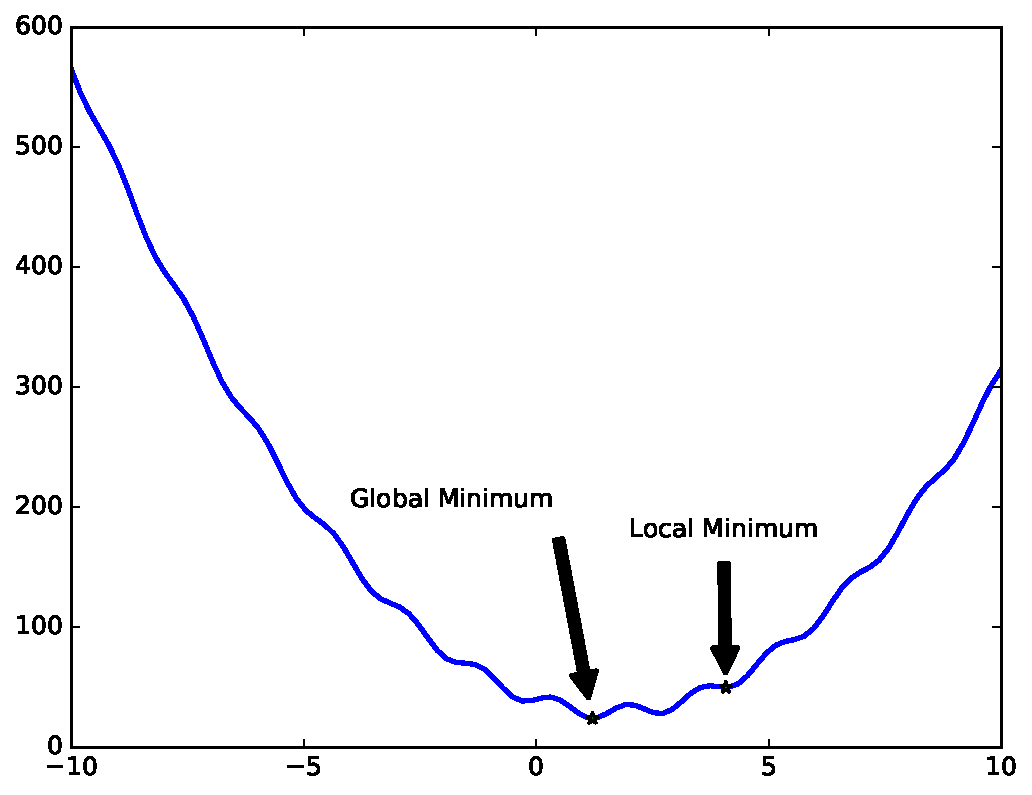
\includegraphics[width=\textwidth]{newton.pdf}
\caption{The results of Newton's Method using two
different initial guess. The global minimizer was
correctly found with initial guess of 1. However,
an initial guess of 4 led to only a local minimum.}
\label{linesearch:newton}
\end{figure}

\begin{problem}
Implement Newton's Method as described using the following function declaration. 
\begin{lstlisting}
def newton1d(f, df, ddf, x, niter=10):
    '''
    Perform Newton's method to minimize a function from R to R.
    
    Parameters
    ----------
    f : callable function object 
        The objective function (twice differentiable)
    df : callable function object 
        The first derivative
    ddf : callable function object
        The second derivative
    x : float
        The initial guess
    niter : integer
        The number of iterations
        
    Returns
    ------
        min : float
            The approximated minimizer
    '''
    pass
\end{lstlisting}

Use this function to minimize $x^2 + \sin(5x)$ with an initial guess of $x_0 = 0$.
Now try other initial guesses farther away from the true minimizer, and note when the
method fails to obtain the correct answer.
\end{problem}

\section*{General Line Search Methods}
\subsection*{Step Size Calculation}
We now examine Line Search methods in more generality. Given a differentiable function
$f : \mathbb{R}^n \rightarrow \mathbb{R}$ that we wish to minimize, and assuming that
we already have a current point $x_k$ and direction $p_k$ in which to search, how do we
choose our step size $\alpha_k$? If our step size is too small, we will not make good progress
toward the minimizer, and convergence will be slow. If the step size is too large, however,
we may overshoot and produce points that are far away from the solution.
A common approach to pick an appropriate step size involves the \emph{Wolfe conditions}:

\begin{align*}
&f(x_k + \alpha_kp_k) \leq f(x_k) + c_1\alpha_k\nabla f_k^Tp_k, &(0 < c_1 < 1),
\\ &\nabla f(x_k + \alpha_kp_k)^Tp_k \geq c_2\nabla f_k^Tp_k, &(c_1 < c_2 < 1).
\end{align*}

Here, we use the shorthand notation $\nabla f_k$ to
mean the gradient of $f$ evaluated at the point $x_k$. The search direction $p_k$ is
often required to satisfy $p_k^T \nabla f_k < 0$, in which case it is called a
\emph{descent direction}, since the function is guaranteed to decrease in
this direction. Generally speaking, choosing a step size $\alpha_k$ satisfying these conditions
ensures that we achieve sufficient decrease in the function and also that we do not
terminate the search at a point of steep decrease (since then we could achieve even
better results by choosing a slightly larger step size). The first condition is known
as the \emph{Armijo} condition.

Finding such a step size satisfying these conditions is not always an easy task, however.
One simple approach, known as \emph{backtracking}, starts with an initial step size
$\alpha$, and repeatedly scales it down until the Armijo condition is satisfied.
That is, choose $\alpha >0, \rho \in (0, 1), c\in (0, 1)$, and while
$$
f(x_k + \alpha p_k) > f(x_k) + c\alpha\nabla f_k^Tp_k,
$$
re-scale $\alpha := \rho\alpha$. Once the loop terminates, set $\alpha_k = \alpha$. Note that the value
$\nabla f_k^Tp_k$ remains fixed for the duration of the backtracking algorithm, and hence need only
be calculated once at the beginning.

\begin{problem}
Implement this backtracking algorithm using the following function declaration. 
\begin{lstlisting}
def backtracking(f, slope, x, p, a=1, rho=.9, c=10e-4):
    '''
    Perform a backtracking line search to satisfy the Armijo condition.
    
    Parameters
    ----------
    f : callable function object
        The objective function
    slope : float 
        The value of grad(f)^T p
    x : ndarray of shape (n,) 
        The current iterate
    p : ndarray of shape (n,) 
        The current search direction
    a : float 
        The intial step length (set to 1 in Newton and quasi-Newton methods)
    rho : float 
        A number in (0,1)
    c : float 
        A number in (0,1)
    
    Returns
    -------
        alpha : float
            The computed step size satisfying the Armijo condition.
    '''
    pass
\end{lstlisting}
\end{problem}


\begin{problem}
Implement the Gradient Descent algorithm and Newton's Method using the following function declarations.
In each function, you should call your backtracking function with
values $\alpha = 1, \rho = .9$, and $c = 10^{-4}$. The \li{scipy.linalg} module
may be useful when computing the search direction in Newton's Method.
\begin{lstlisting}
def gradientDescent(f, df, x, niter=10):
    '''
    Minimize a function using gradient descent.
    
    Parameters
    ----------
    f : callable function object 
        A differentiable real-valued function
    df : callable function object 
        The gradient of the function
    x : ndarray of shape (n,) 
        The initial point
    niter : integer 
        The number of iterations to run.
    
    Returns
    -------
        pts: list of ndarrays 
            The sequence of points generated
    '''
    pass

def newtonsMethod(f, df, ddf, x, niter=10):
    '''
    Minimize a function using Newton's method.
    
    Parameters
    ----------
    f : callable function object
        Real-valued, twice-differentiable function
    df : callable function object
        The gradient of the function
    ddf : callable function object 
        The Hessian of the function
    x : ndarray of shape (n,) 
        The initial point
    niter : integer 
        The number of iterations
        
    Returns
    -------
    pts : list of ndarrays
        The sequence of points generated
    '''
    pass
\end{lstlisting}

\end{problem}

\subsection*{Line Search in SciPy}
The SciPy module \li{scipy.optimize} contains implementations of various optimization algorithms,
including several line search methods. In particular, the module provides a useful routine for
calculating a step size satisfying the Wolfe Conditions described above, which is more robust
and efficient than our simple backtracking approach. We recommend its use for the remainder of
this lab. The function is called \li{line_search}, and accepts several arguments. We can typically
leave the keyword arguments at their default values, but we do need to pass in the objective
function, its gradient, the current point, and the search direction. The following code gives
an example of its usage, using the objective function $f(x, y) = x^2+4y^2$.
\begin{lstlisting}
>>> import numpy as np
>>> from scipy.optimize import line_search
>>>
>>> def objective(x):
>>>     return x[0]**2 + 4*x[1]**2
>>>
>>> def grad(x):
>>>     return 2*x*np.array([1, 4])
>>>
>>> x = np.array([1., 3.]) #current point
>>> p = -grad(x)           #current search direction
>>> a = line_search(objective, grad, x, p)[0]
>>> print a
0.125649913345
\end{lstlisting}
Note that the function returns a tuple of values, the first of which is the step size. We have illustrated
the very basic use of this function. See the documentation for further uses.
